\section{Experiments}

\begin{figure*}[!t]
 \centering
 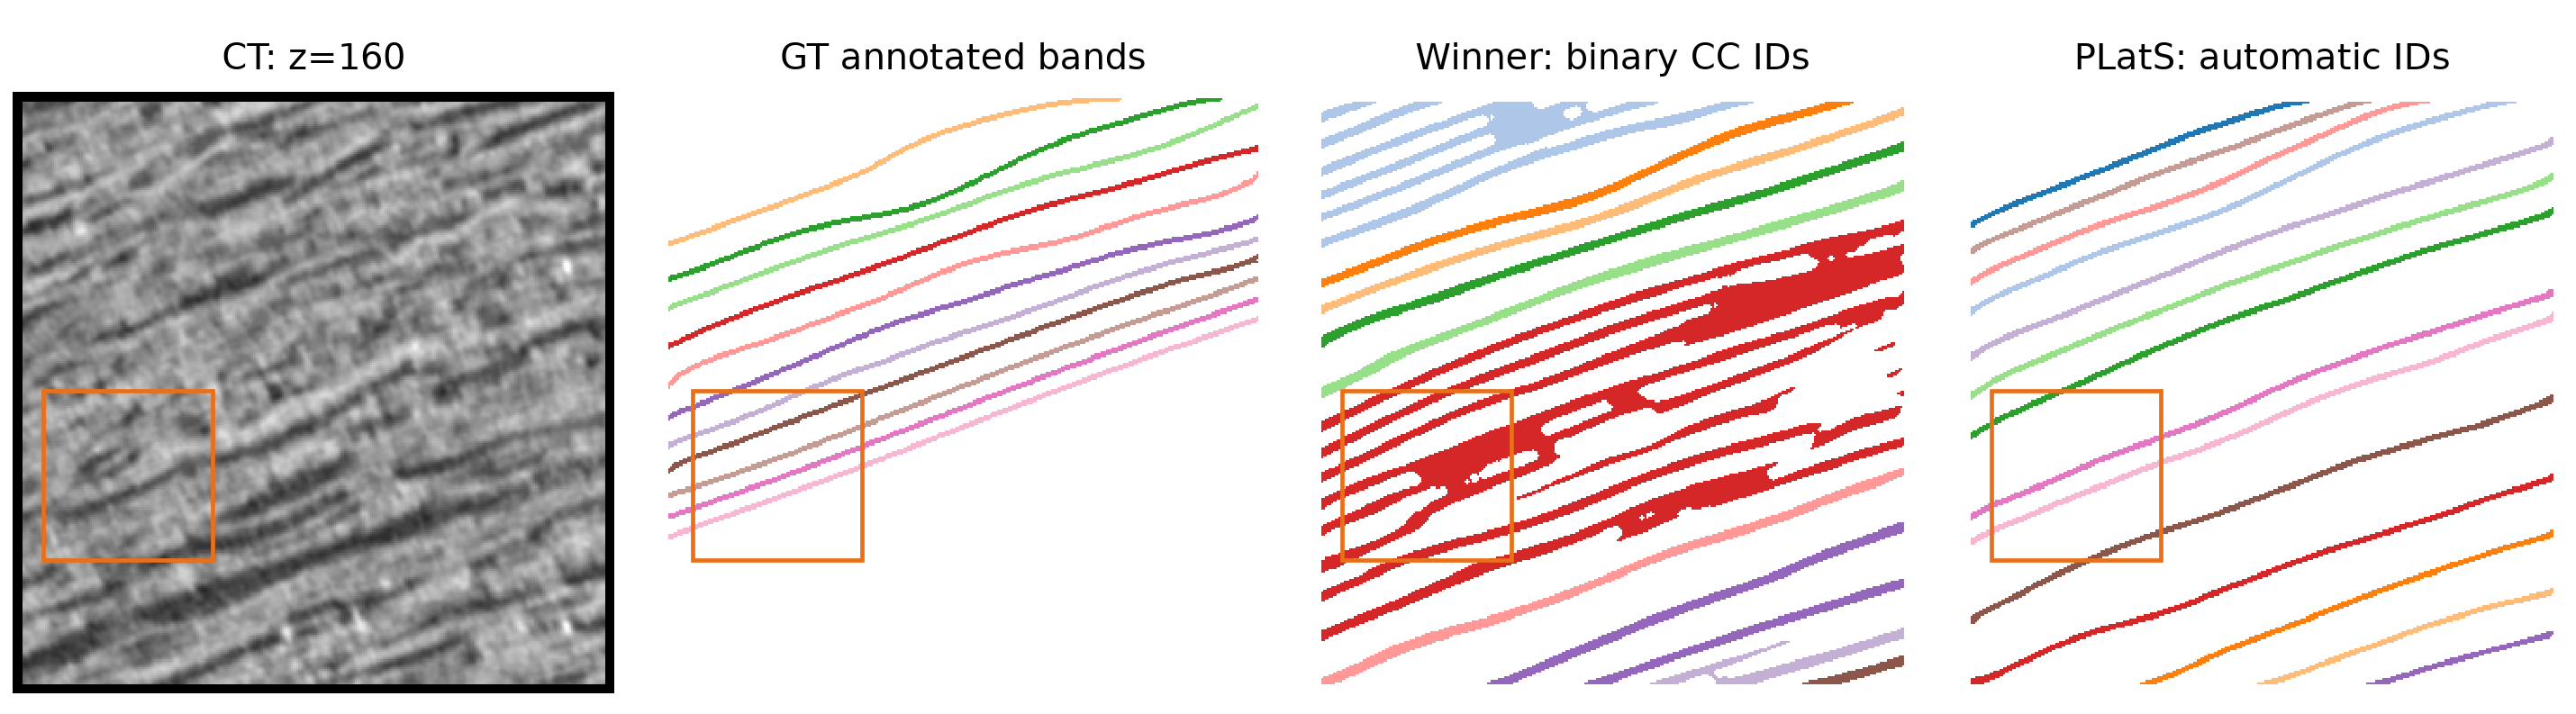
\includegraphics[width=\textwidth]{figures/binary_failure_main.png}
 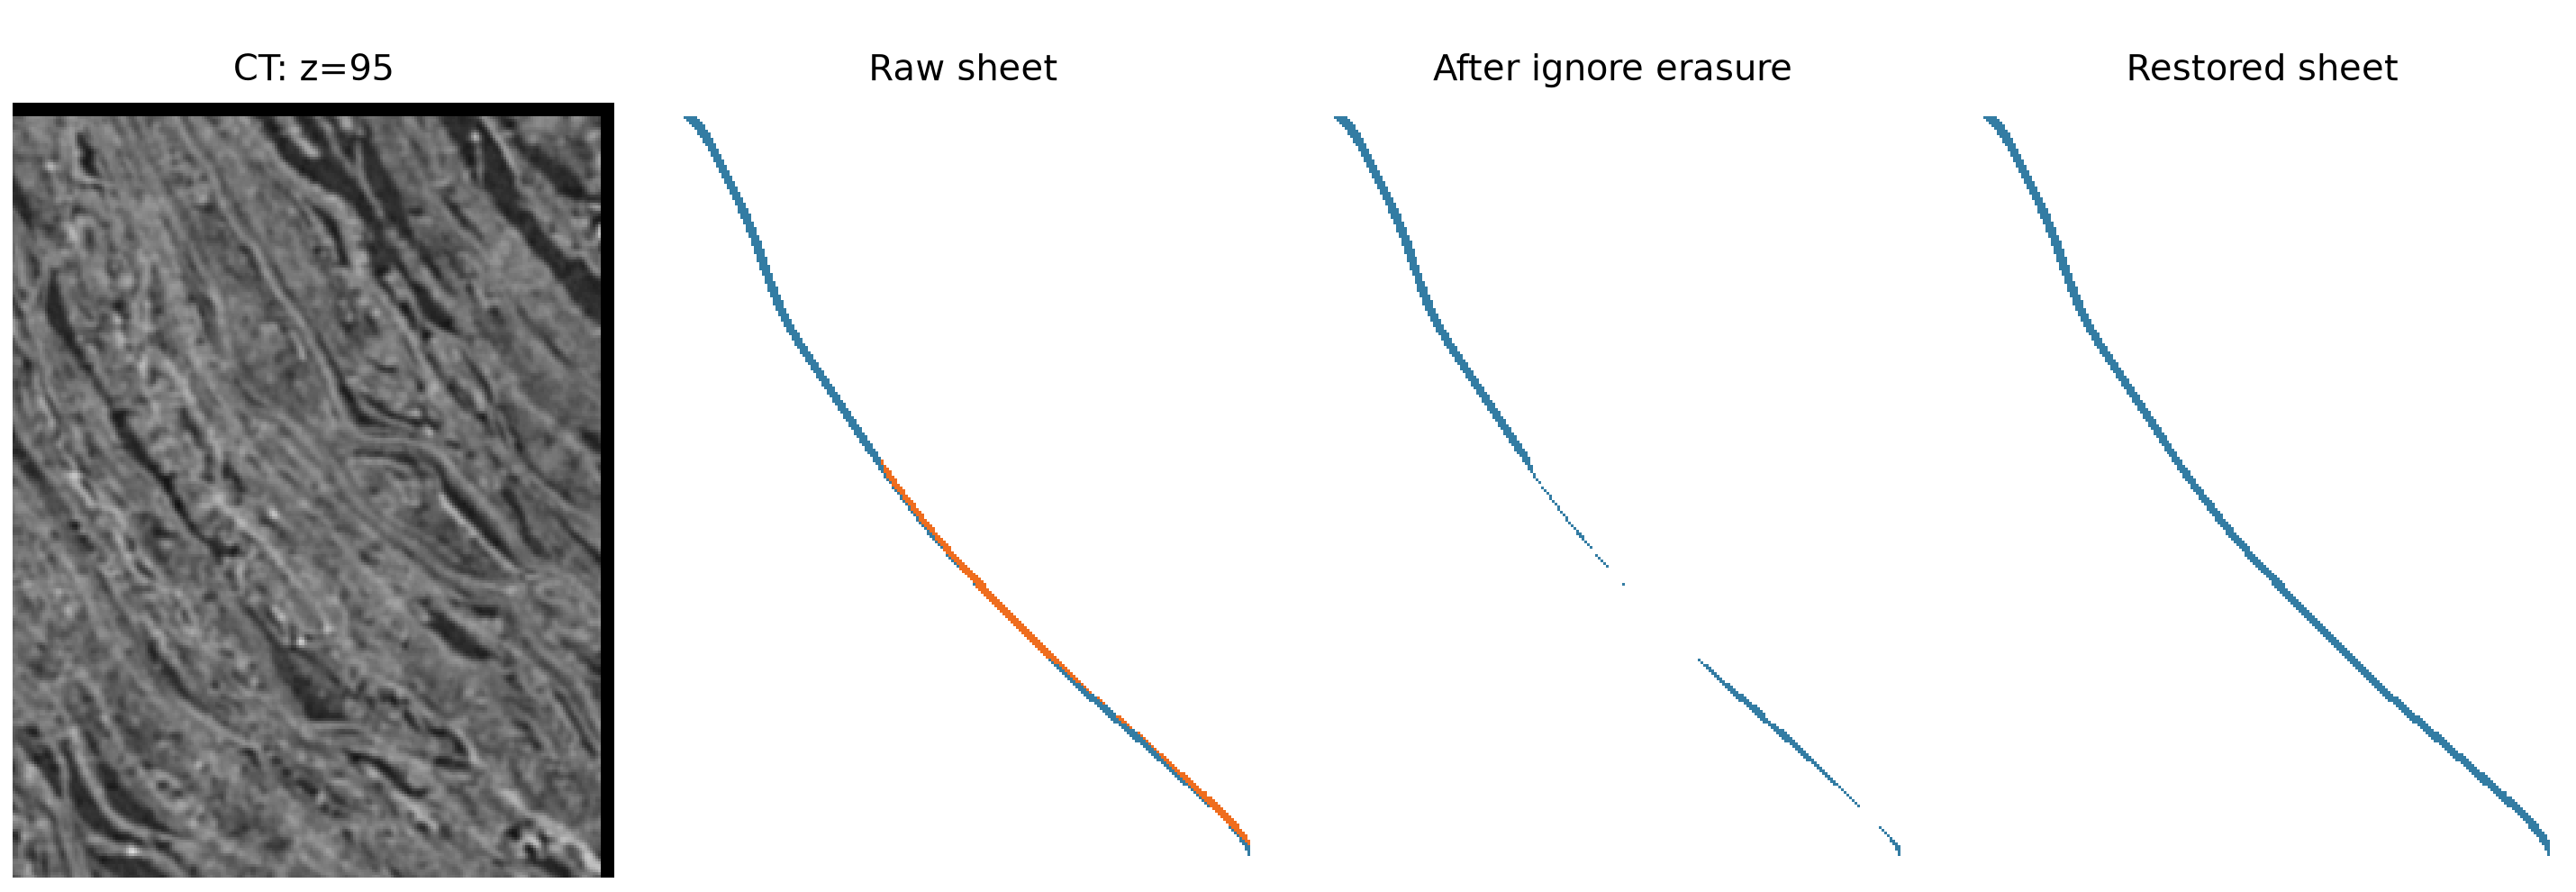
\includegraphics[width=\textwidth]{figures/ignore_failure.png}
 \caption{\textbf{Two different topology failures.}
 Top: a winner component joins six annotated bands in case 00860 ($z=160$);
 Base PLatS preserves gaps but misses bands. Colors are IDs within each method.
 Bottom: ignore erasure cuts a predicted sheet in case 00829 ($z=95$).
 Its whole-volume topology changes from one component and no tunnels to
 495 components and 1,023 tunnels. Restoring its own voxels reverses the cuts.
 Orange marks removed voxels. Both rows use native $z$ slices; selection
 rules and the enlarged orange-square crop are in Supplementary.}
 \label{fig:binary}\label{fig:ignore}
\end{figure*}

\begin{figure*}[!t]
 \centering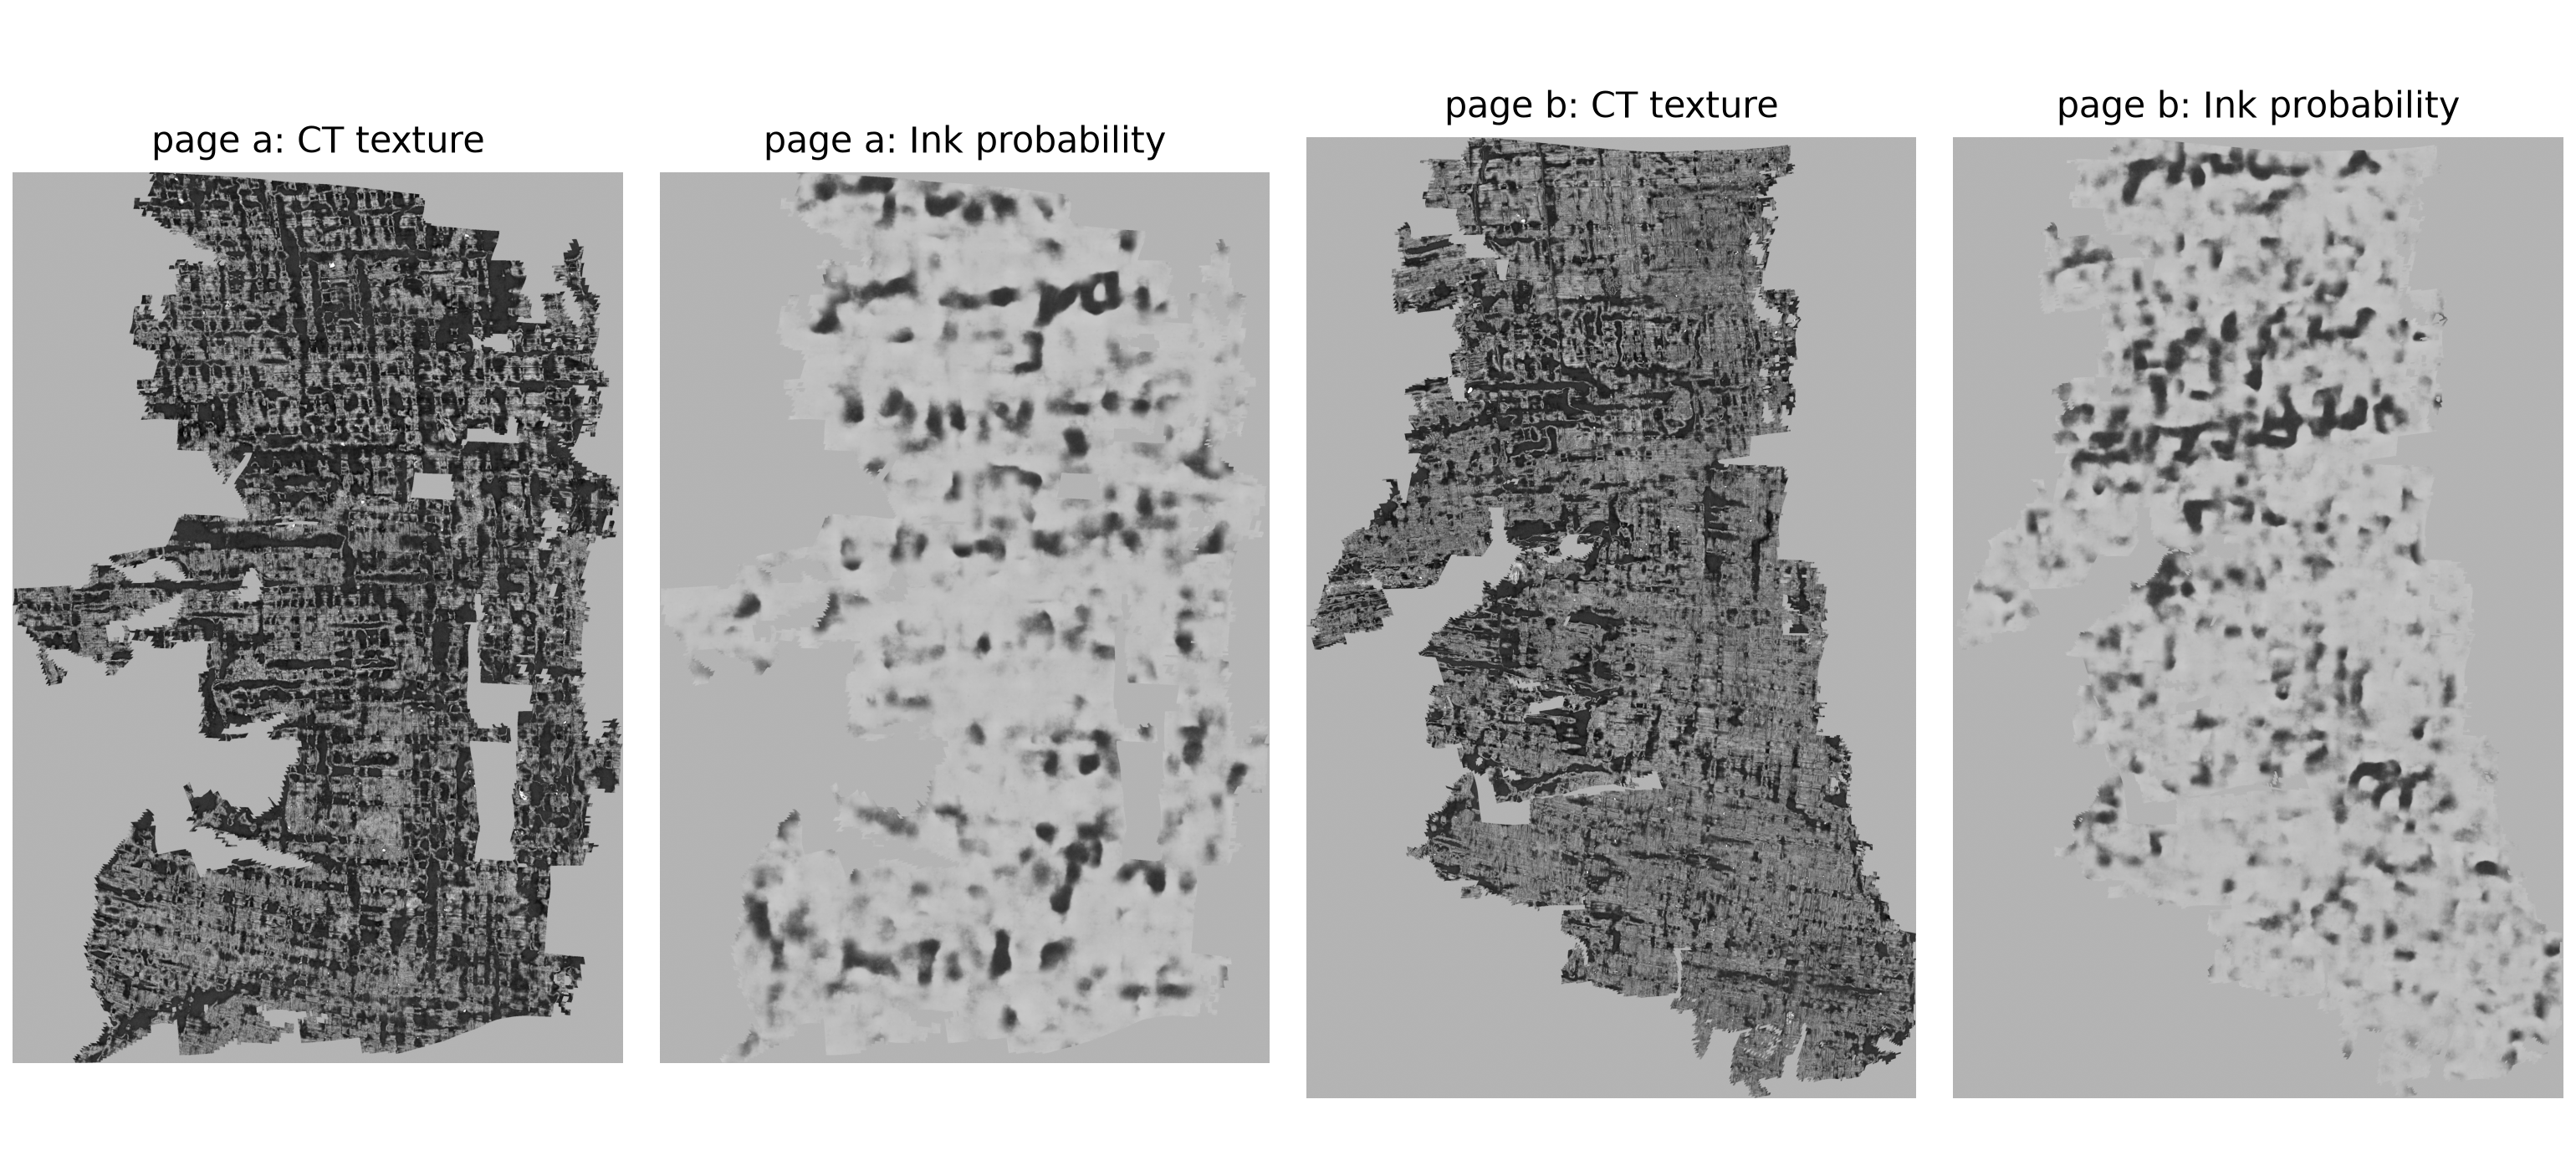
\includegraphics[width=\textwidth]{figures/large_ink.png}
 \caption{\textbf{Centimeter-scale surfaces and ink.} Independently flattened
 CT texture and ink probabilities from PLatS on two PHerc0139 regions.
 Darker ink pixels indicate higher probability. Whole charts expose gaps and
 stitching limitations; native PNGs accompany the report.}
 \label{fig:largeink}
\end{figure*}
\label{sec:experiments}

\paragraph{Setup.}
We use Kaggle-only checkpoint \textbf{0058} for the main comparisons and
evaluate all \textbf{106 released test cubes}. Training-case IDs are excluded,
but labels are now public and some crops were previously inspected; this is
not a fresh blind submission. External-data checkpoints, training details and
all 1/2/4/8-point results are in Supplementary. We evaluate automatic union
quality, ignore-erasure sensitivity, prompted geometry and identity, then
downstream surfaces. The base automatic benchmark fixes a separate
foreground proposer across checkpoints; these saved predictions appear in
Fig.~\ref{fig:inference}. The co-trained proposal path and new scratch recipe
have no accuracy results here.

\subsection{Binary segmentation and topology}
We first apply the original leaderboard protocol: erase source-ignore voxels
from prediction and GT, then compute the public formula~\cite{vesuviuseval}:
\begin{equation}
 J=0.35\,\mathrm{SD}_2+0.30\,\mathrm{Topo}+0.35\,\mathrm{VOI}.
 \label{eq:formula}
\end{equation}
$J$ is the combined score, $\mathrm{SD}_2$ Surface Dice at two voxels,
$\mathrm{Topo}$ exact matched TopoScore~\cite{stucki2022betti}, and
$\mathrm{VOI}$ the public variation-of-information score.
Table~\ref{tab:lb} compares the released winner with automatic PLatS,
using no GT prompts and equal weight per cube.

\begin{table}[t]
\centering
\small
\setlength{\tabcolsep}{3pt}
\begin{tabular}{lrrrrr}
\toprule
Method & Dice & SD$_2$ & Topo & VOI & LB \\
\midrule
Winner & 0.6015 & 0.8799 & 0.3769 & 0.5616 & 0.6176 \\
PLatS & 0.4262 & 0.7494 & 0.2644 & 0.5396 & 0.5305 \\
PLatS + repair & 0.4237 & 0.7487 & 0.2742 & 0.5393 & 0.5331 \\
\bottomrule
\end{tabular}
\caption{Original source-ignore erasure on all 106 released test cubes. Equal-case means; automatic inference, no GT prompts. Repair adds AE reconstruction, guarded closing and dusting before erasure. LB is reproduced locally.}
\label{tab:lb}
\end{table}


Without added repair, the winner scores 0.6176 versus 0.5305 for PLatS.
AE reconstruction, guarded per-sheet closing and tiny-component dusting change
PLatS to 0.5331. The topology gain offsets small Dice and Surface Dice losses.
Supplementary separates these steps and adds a winner
cleanup control. Binary masks can still join distinct sheets
(Fig.~\ref{fig:binary}, top); PLatS separates layers there while missing bands.
The example illustrates a failure mode, rather than establishing superiority.

\subsection{Separating ignore cuts from model defects}
Erasing ignored labels can create holes in an otherwise continuous prediction
(Fig.~\ref{fig:ignore}, bottom). We therefore also report an
\emph{ignore-restoration diagnostic}: restore cut instances from their own
pre-erasure predictions, exclude entirely ignored instances, and remove
instances smaller than 5,000 voxels \emph{after restoration}.
The winner's identities are raw connected components; PLatS provides sheet IDs.
GT remains erased. Table~\ref{tab:modified} uses the same three formula terms.
This is \emph{not an official leaderboard score}: restored unknown foreground
can still incur penalties. The exact rule and filtering controls are in
Supplementary.

\begin{table}[t]
\centering
\small
\setlength{\tabcolsep}{3pt}
\begin{tabular}{lrrrrr}
\toprule
Method & Dice & SD$_2$ & Topo & VOI & LB \\
\midrule
Winner & 0.5460 & 0.8078 & 0.5694 & 0.5719 & 0.6537 \\
PLatS & 0.4046 & 0.7120 & 0.5820 & 0.5390 & 0.6124 \\
PLatS + repair & 0.4019 & 0.7103 & 0.6364 & 0.5386 & 0.6280 \\
\bottomrule
\end{tabular}
\caption{Restoration diagnostic on the same 106 cases, using the full-size 5,000-voxel instance gate. All terms use restored predictions and erased GT. Repair precedes restoration. This is not official LB.}
\label{tab:modified}
\end{table}

Restoration gives 0.6537 for the winner, 0.6124 for base PLatS and
0.6280 for repaired PLatS. Its repaired topology term is 0.6364.
This diagnoses erasure sensitivity and postprocessing effects;
it does not establish a new challenge ranking.

\paragraph{Topology before ignore processing.}
Table~\ref{tab:rawpredbetti} counts whole-union tunnels ($b_1$) and cavities
($b_2$), including unannotated regions. Repair reduces mean tunnels from
34.849 to 23.321 and cavities from 7.972 to 4.802, but union defects remain. Counts describe
prediction topology, not errors against GT or spatially matched TopoScores.

\begin{table}[t]
\centering
\small
\setlength{\tabcolsep}{5pt}
\begin{tabular}{lrrrr}
\toprule
 & \multicolumn{2}{c}{$b_1$: tunnels} & \multicolumn{2}{c}{$b_2$: cavities} \\
Method & Mean & Median & Mean & Median \\
\midrule
Winner & 40.302 & 20.5 & 0.000 & 0.0 \\
PLatS & 34.849 & 2.5 & 7.972 & 0.0 \\
\bottomrule
\end{tabular}
\caption{Raw binary prediction unions on the same 106 native crops as
Tables~\ref{tab:lb}--\ref{tab:modified}. Whole-volume Betti counts use
V construction (six-connected foreground), with equal weight per case.
No ignore erasure, restoration or additional size filtering is applied;
each method's existing inference postprocessing is retained.}
\label{tab:rawpredbetti}
\end{table}


\subsection{Sheet geometry and latent identity}
To separate representation quality from automatic seed selection, we use
nested GT prompts on 764 eligible annotated bands. Before cleanup or ignore
erasure, 87.3\% of eight-point predictions have one component and no tunnels
or cavities. This is a topology statistic, not a geometric correctness rate.
Table~\ref{tab:promptmain} measures alignment: increasing prompts from one to
eight raises Surface Dice from 0.7689 to 0.8058, while voxel Dice remains modest.
GT components and repaired training targets favor simple sheet topology.

\begin{table}[t]
\centering
\small
\setlength{\tabcolsep}{4pt}
\begin{tabular}{lrrrrr}
\toprule
Points & Dice & SD$_2$ & Topo & VOI & Formula \\
\midrule
1 & 0.4314 & 0.7689 & 0.6864 & 0.7502 & 0.7376 \\
8 & 0.4517 & 0.8058 & 0.7045 & 0.7440 & 0.7538 \\
\bottomrule
\end{tabular}
\caption{Prompted 0058 sheets with no cleanup. Only the exterior of the
annotated-region box is ignored; internal unannotated voxels are background.
All three formula terms are shown. This policy and GT prompts differ from
the automatic original-erasure comparison in Table~\ref{tab:lb}.}
\label{tab:promptmain}
\end{table}


For 6,112 single-point codes, same-band versus different-band classification
has 0.9121 AUROC. The distributions overlap: at the inherited MSE threshold
0.02, 50.03\% of same-band pairs exceed it. Base automatic instance accuracy,
TP/(TP+FP+FN), is 0.420 at IoU 0.25 but only 0.071 at IoU 0.50.
Useful code separation therefore coexists with clustering and alignment errors.
Supplementary reports complete prompt counts, instance diagnostics and raw
topology; none is a causal ablation of the AE or identity losses.

\subsection{From sheets to ink}
Predictions are meshed, independently flattened, and passed to a frozen ink
model~\cite{scrollfiesta,rabinovich2017slim,scrollprizeink}.
Figure~\ref{fig:largeink} shows two PHerc0139 regions of approximately
$20\times33$ and $23\times44$~mm. Each begins with one published-track point
and grows using predicted points; reference layouts and ink labels are
excluded from reconstruction. Median accepted join distances are 1.181 and
1.361 voxels, versus reference-distance p90 values of 15.856 and 15.234 voxels:
local continuity does not ensure global alignment. Page A covers 17.37\% of
annotated pixels. Gaps and diffuse ink remain. These outputs demonstrate the
pipeline, not new text recovery; the ink model's training includes this scroll.
